% tpaxos-refinement.tex

\documentclass[tikz]{standalone}
\usetikzlibrary{positioning, arrows.meta, fit}

\begin{document}
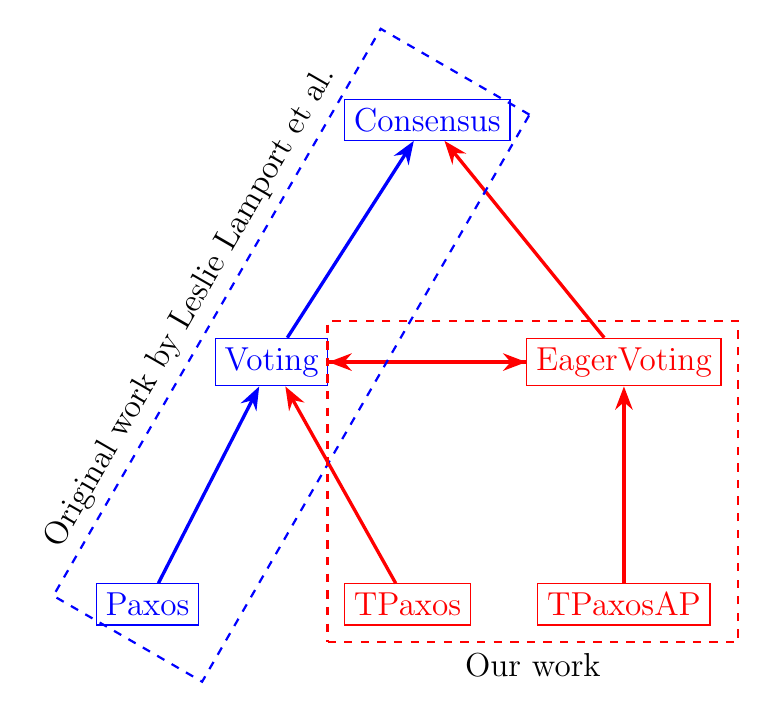
\begin{tikzpicture}[every node/.style = {draw, rectangle, font = \large},
  node distance = 2.5cm and 0.2cm,
  every edge/.style = {draw, ->, >=Stealth, very thick}]
  \node (c) [blue] {Consensus};
  \node (v) [below left = of c, blue] {Voting};
  \node (ev) [below right = of c, red] {EagerVoting};
  \node (paxos) [below left = of v, blue] {Paxos};
  \node (tpaxos) [below right = of v, red] {TPaxos};
  \node (tpaxosap) [below = of ev, red] {TPaxosAP};

  \path (paxos) edge[blue] (v)
	(v) edge[blue] (c)
	(tpaxos) edge[red] (v)
	(tpaxosap) edge[red] (ev)
	(ev) edge[red] (c)
	(v) edge[red] (ev)
	(ev) edge[red] (v);

  \node () [rotate fit = -30, thick, dashed, blue, fit = (c) (v) (paxos), inner sep = 5pt,
    label = {[rotate = 60, xshift = 3.50cm, font = \large] left : Original work by Leslie Lamport et al.}] {};

  \node () [thick, dashed, red, fit = (ev) (tpaxos) (tpaxosap), inner sep = 6pt,
    label = {[font = \large] below : Our work}] {};
\end{tikzpicture}
\end{document}